\documentclass[border=10pt]{standalone}
\usepackage[utf8]{inputenc}
\usepackage{tikz}
\usetikzlibrary{shapes,arrows,positioning}

\tikzset{
  class/.style = {
    rectangle,
    draw=black,
    line width=1.5pt,
    font=\small,
    text width=3.2cm,
    inner sep=5pt,
    text centered
  },
  uml_arrow/.style = {
    thick,
    ->,
    >=stealth
  },
  uml_dashed/.style = {
    thick,
    ->,
    >=stealth,
    dashed
  }
}

\begin{document}

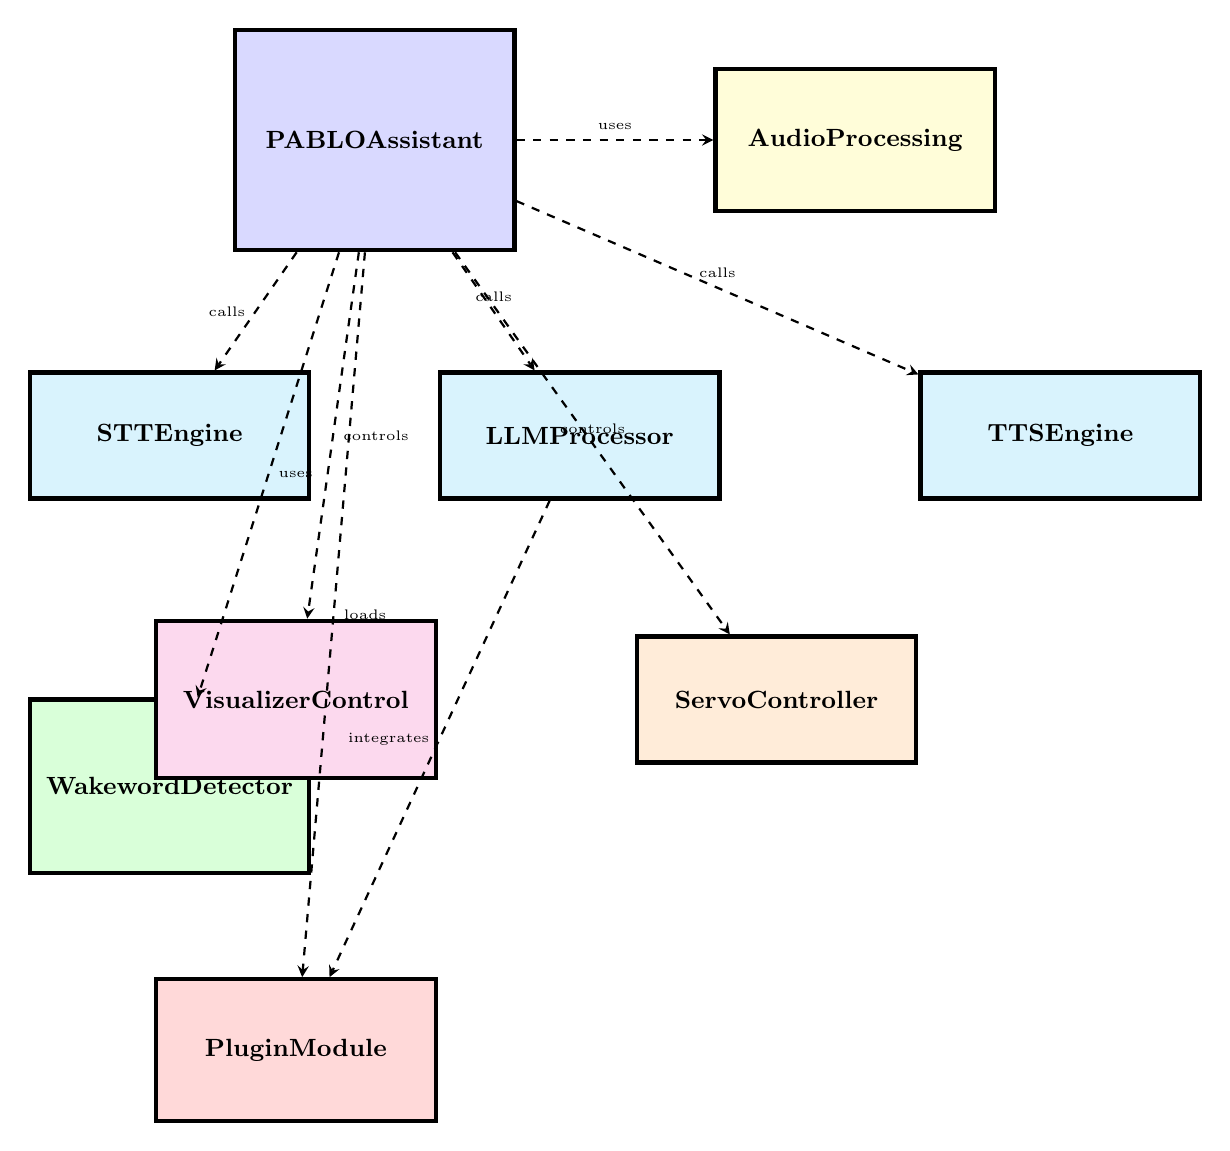
\begin{tikzpicture}[node distance=2.5cm]

% PABLOAssistant - Zentrale Klasse
\node[class, minimum height=2.8cm, fill=blue!15] (main) {
  \textbf{PABLOAssistant}
  \nodepart{two}
  config: dict
  modules: list
  detector: WakewordAngleDetector
  visualizer\_queue: Queue
  \nodepart{three}
  main()
  process\_audio(): str
  process\_llm(): dict
};

% Audio-Utility
\node[class, minimum height=1.8cm, fill=yellow!15, right=of main] (util) {
  \textbf{AudioProcessing}
  \nodepart{two}
  SERVO\_LEFT: float
  SERVO\_CENTER: float
  \nodepart{three}
  clamp(): float
  voice\_angle\_to\_servo(): float
};

% STT Engine
\node[class, minimum height=1.6cm, fill=cyan!15, below left=1.5cm and -1cm of main] (stt) {
  \textbf{STTEngine}
  \nodepart{two}
  engine: Vosk
  \nodepart{three}
  get\_voice\_input(): str
};

% LLM Processor
\node[class, minimum height=1.6cm, fill=cyan!15, below right=1.5cm and -1cm of main] (llm) {
  \textbf{LLMProcessor}
  \nodepart{two}
  modules: list
  \nodepart{three}
  get\_response(text): dict
};

% TTS Engine
\node[class, minimum height=1.6cm, fill=cyan!15, right=of llm] (tts) {
  \textbf{TTSEngine}
  \nodepart{two}
  engine: Piper
  \nodepart{three}
  speak(text): bool
};

% Wakeword Detector
\node[class, minimum height=2.2cm, fill=green!15, below=of stt] (wakeword) {
  \textbf{WakewordDetector}
  \nodepart{two}
  access\_key: str
  mic\_index: int
  \nodepart{three}
  wait\_and\_locate(): Metrics
  cleanup()
};

% Visualizer Control
\node[class, minimum height=2cm, fill=magenta!15, below left=1.5cm and 0cm of llm] (viz) {
  \textbf{VisualizerControl}
  \nodepart{two}
  state\_queue: Queue
  process: Process
  \nodepart{three}
  start(): Queue
  set\_state(state)
  shutdown()
};

% Servo Controller
\node[class, minimum height=1.6cm, fill=orange!15, right=of viz] (servo) {
  \textbf{ServoController}
  \nodepart{two}
  port: str
  \nodepart{three}
  set\_angle(angle): bool
};

% Plugin Module
\node[class, minimum height=1.8cm, fill=red!15, below=of viz] (plugin) {
  \textbf{PluginModule}
  \nodepart{two}
  name: str
  \nodepart{three}
  execute(command): dict
  get\_help(): str
};

% Verbindungen
\draw[uml_dashed] (main) -- (util) node[midway, above, font=\tiny] {uses};
\draw[uml_dashed] (main) -- (stt) node[midway, left, font=\tiny] {calls};
\draw[uml_dashed] (main) -- (llm) node[midway, above, font=\tiny] {calls};
\draw[uml_dashed] (main) -- (tts) node[midway, above, font=\tiny] {calls};
\draw[uml_dashed] (main) -- (wakeword) node[midway, right, font=\tiny] {uses};
\draw[uml_dashed] (main) -- (viz) node[midway, right, font=\tiny] {controls};
\draw[uml_dashed] (main) -- (servo) node[midway, above, font=\tiny] {controls};
\draw[uml_dashed] (main) -- (plugin) node[midway, right, font=\tiny] {loads};

\draw[uml_dashed] (llm) -- (plugin) node[midway, left, font=\tiny] {integrates};

\end{tikzpicture}

\end{document}
